\begin{frame}
\frametitle{PCE training in the morning}
\begin{columns}[c] % The "c" option specifies centered vertical alignment while the "t" option is used for top vertical alignment

\column{.3\textwidth} % Left column and width
%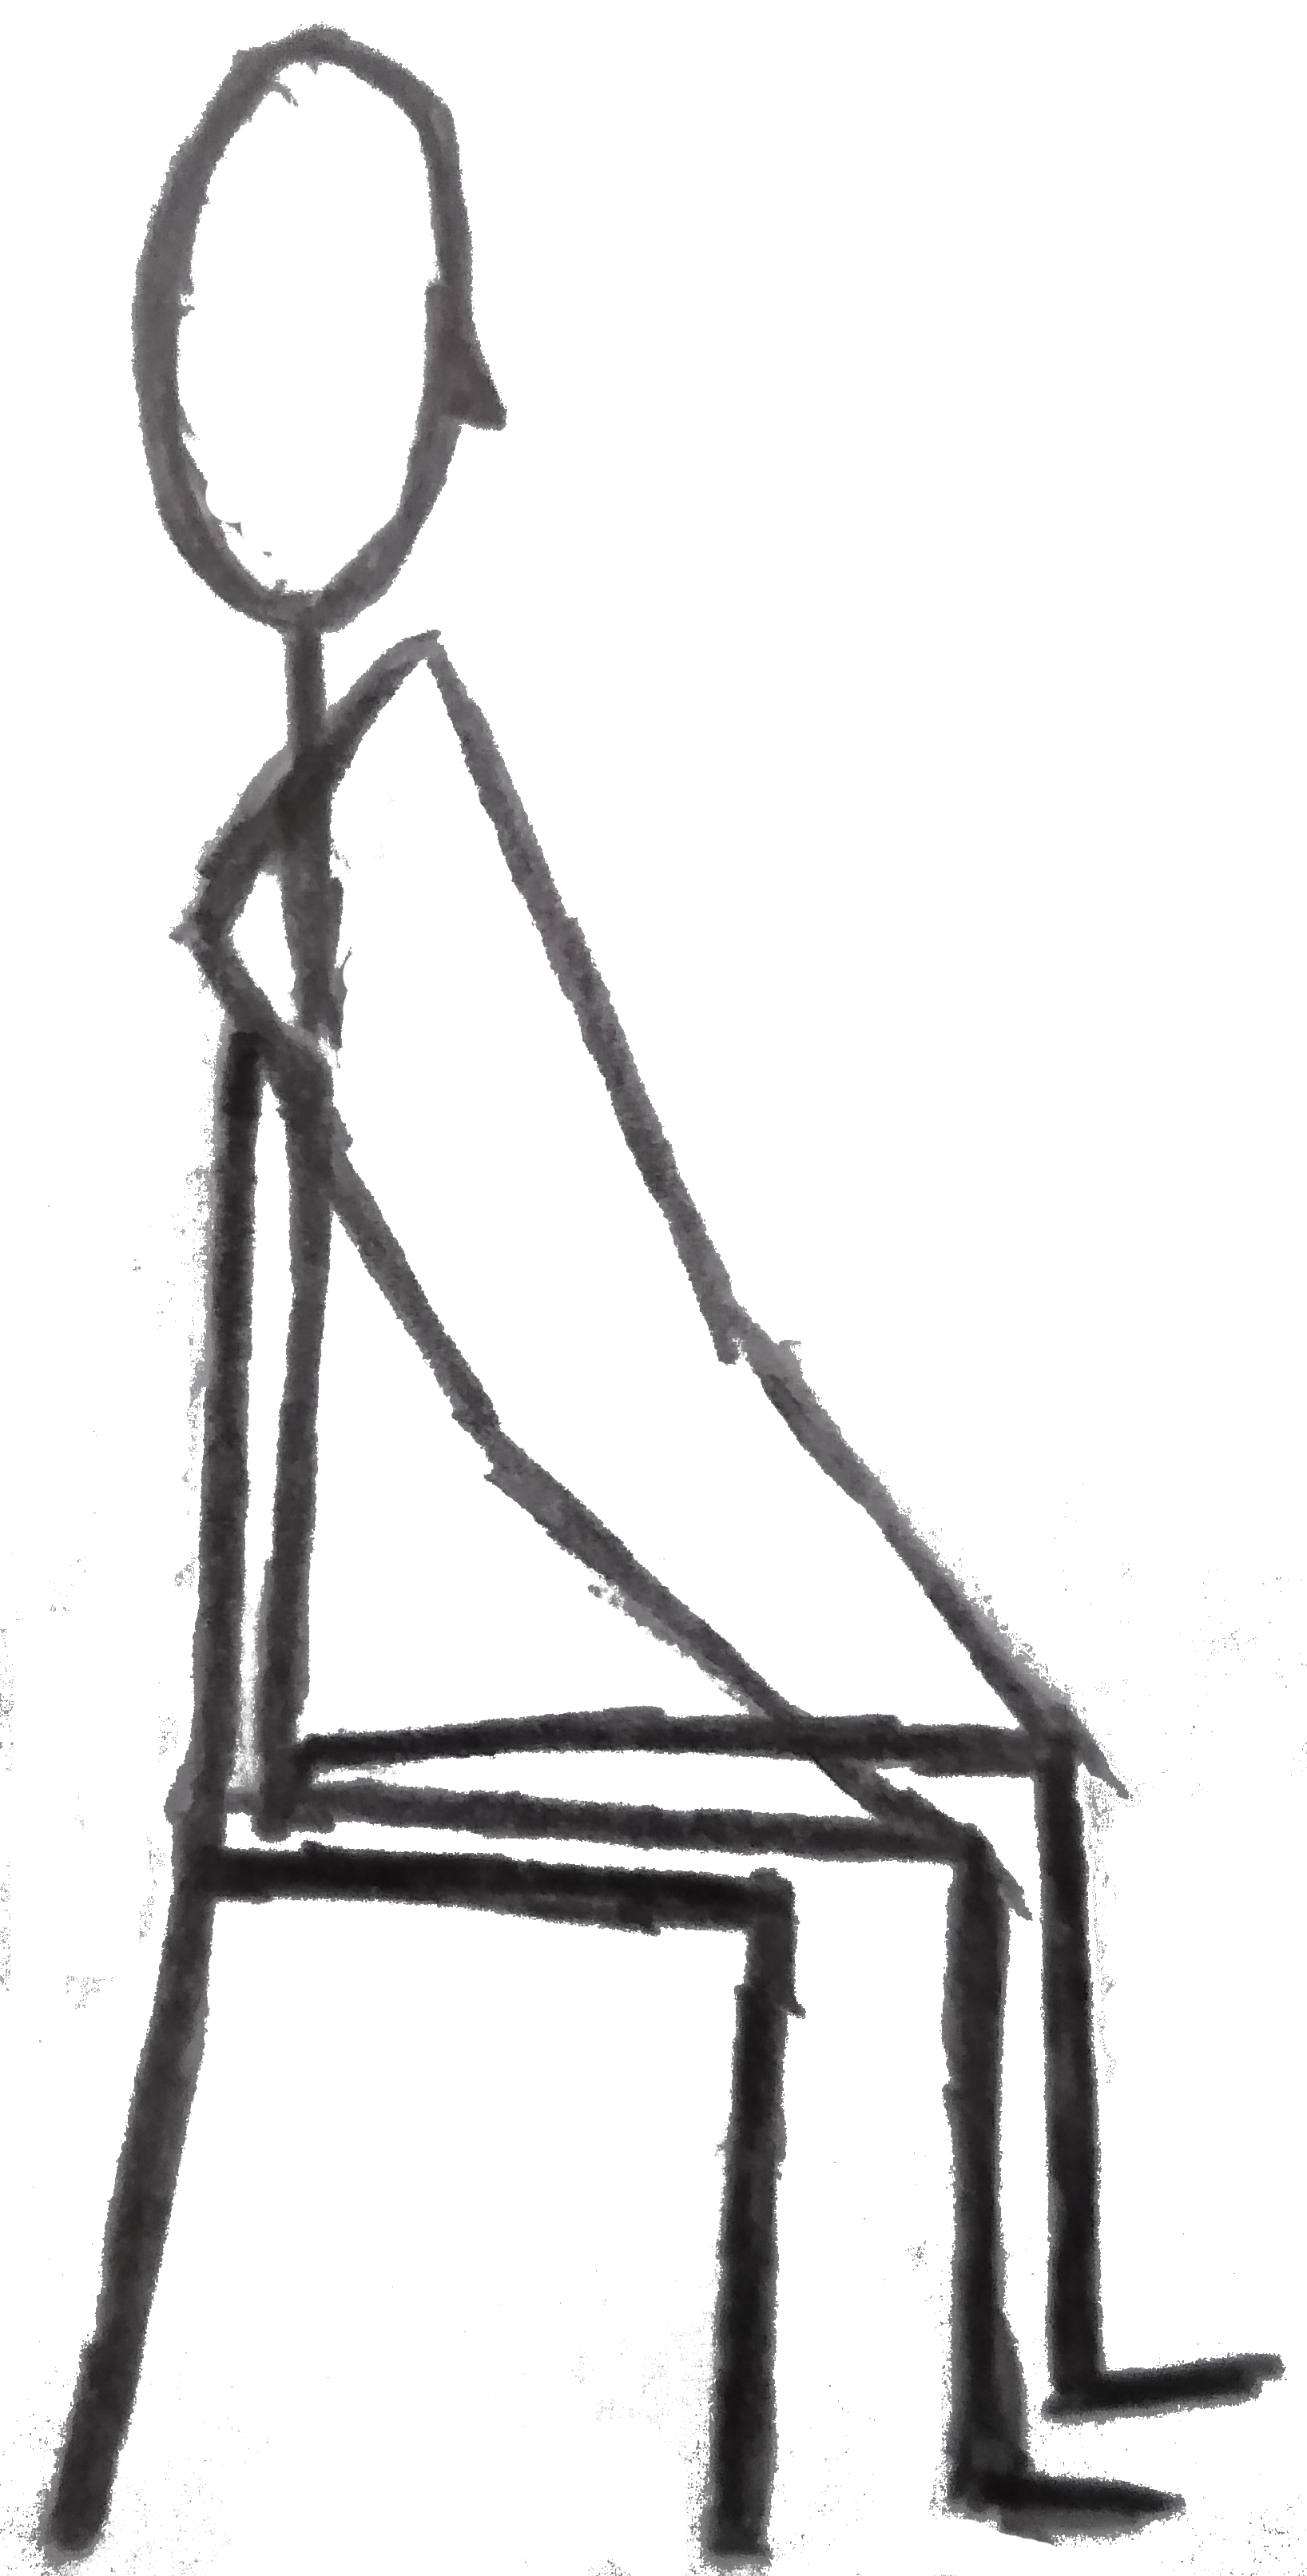
\includegraphics[width=\linewidth]{Sitting_chair_side.png}
\column{.7\textwidth} % Right column and width
\begin{itemize}
\item[-] Chases the \structure{morning rigidity} away form body and soul.
\item[-] The \structure{glands} come back into \structure{harmony}.
\item[-] \structure{Healing energy} can reach all the cells.
\item[-] Body and soul \structure{rejuvenate}.
\item[-] Promotes \structure{creativity}. 
\item[-] A feeling of \structure{joy, happiness and passion} emerges.
\end{itemize}
% Write on
\end{columns}
\end{frame}
%--------------------------------------------------------------------------------------------------------------
\begin{frame}
\frametitle{PCE training in the evening}
\begin{columns}[c] % The "c" option specifies centered vertical alignment while the "t" option is used for top vertical alignment

\column{.3\textwidth} % Left column and width
%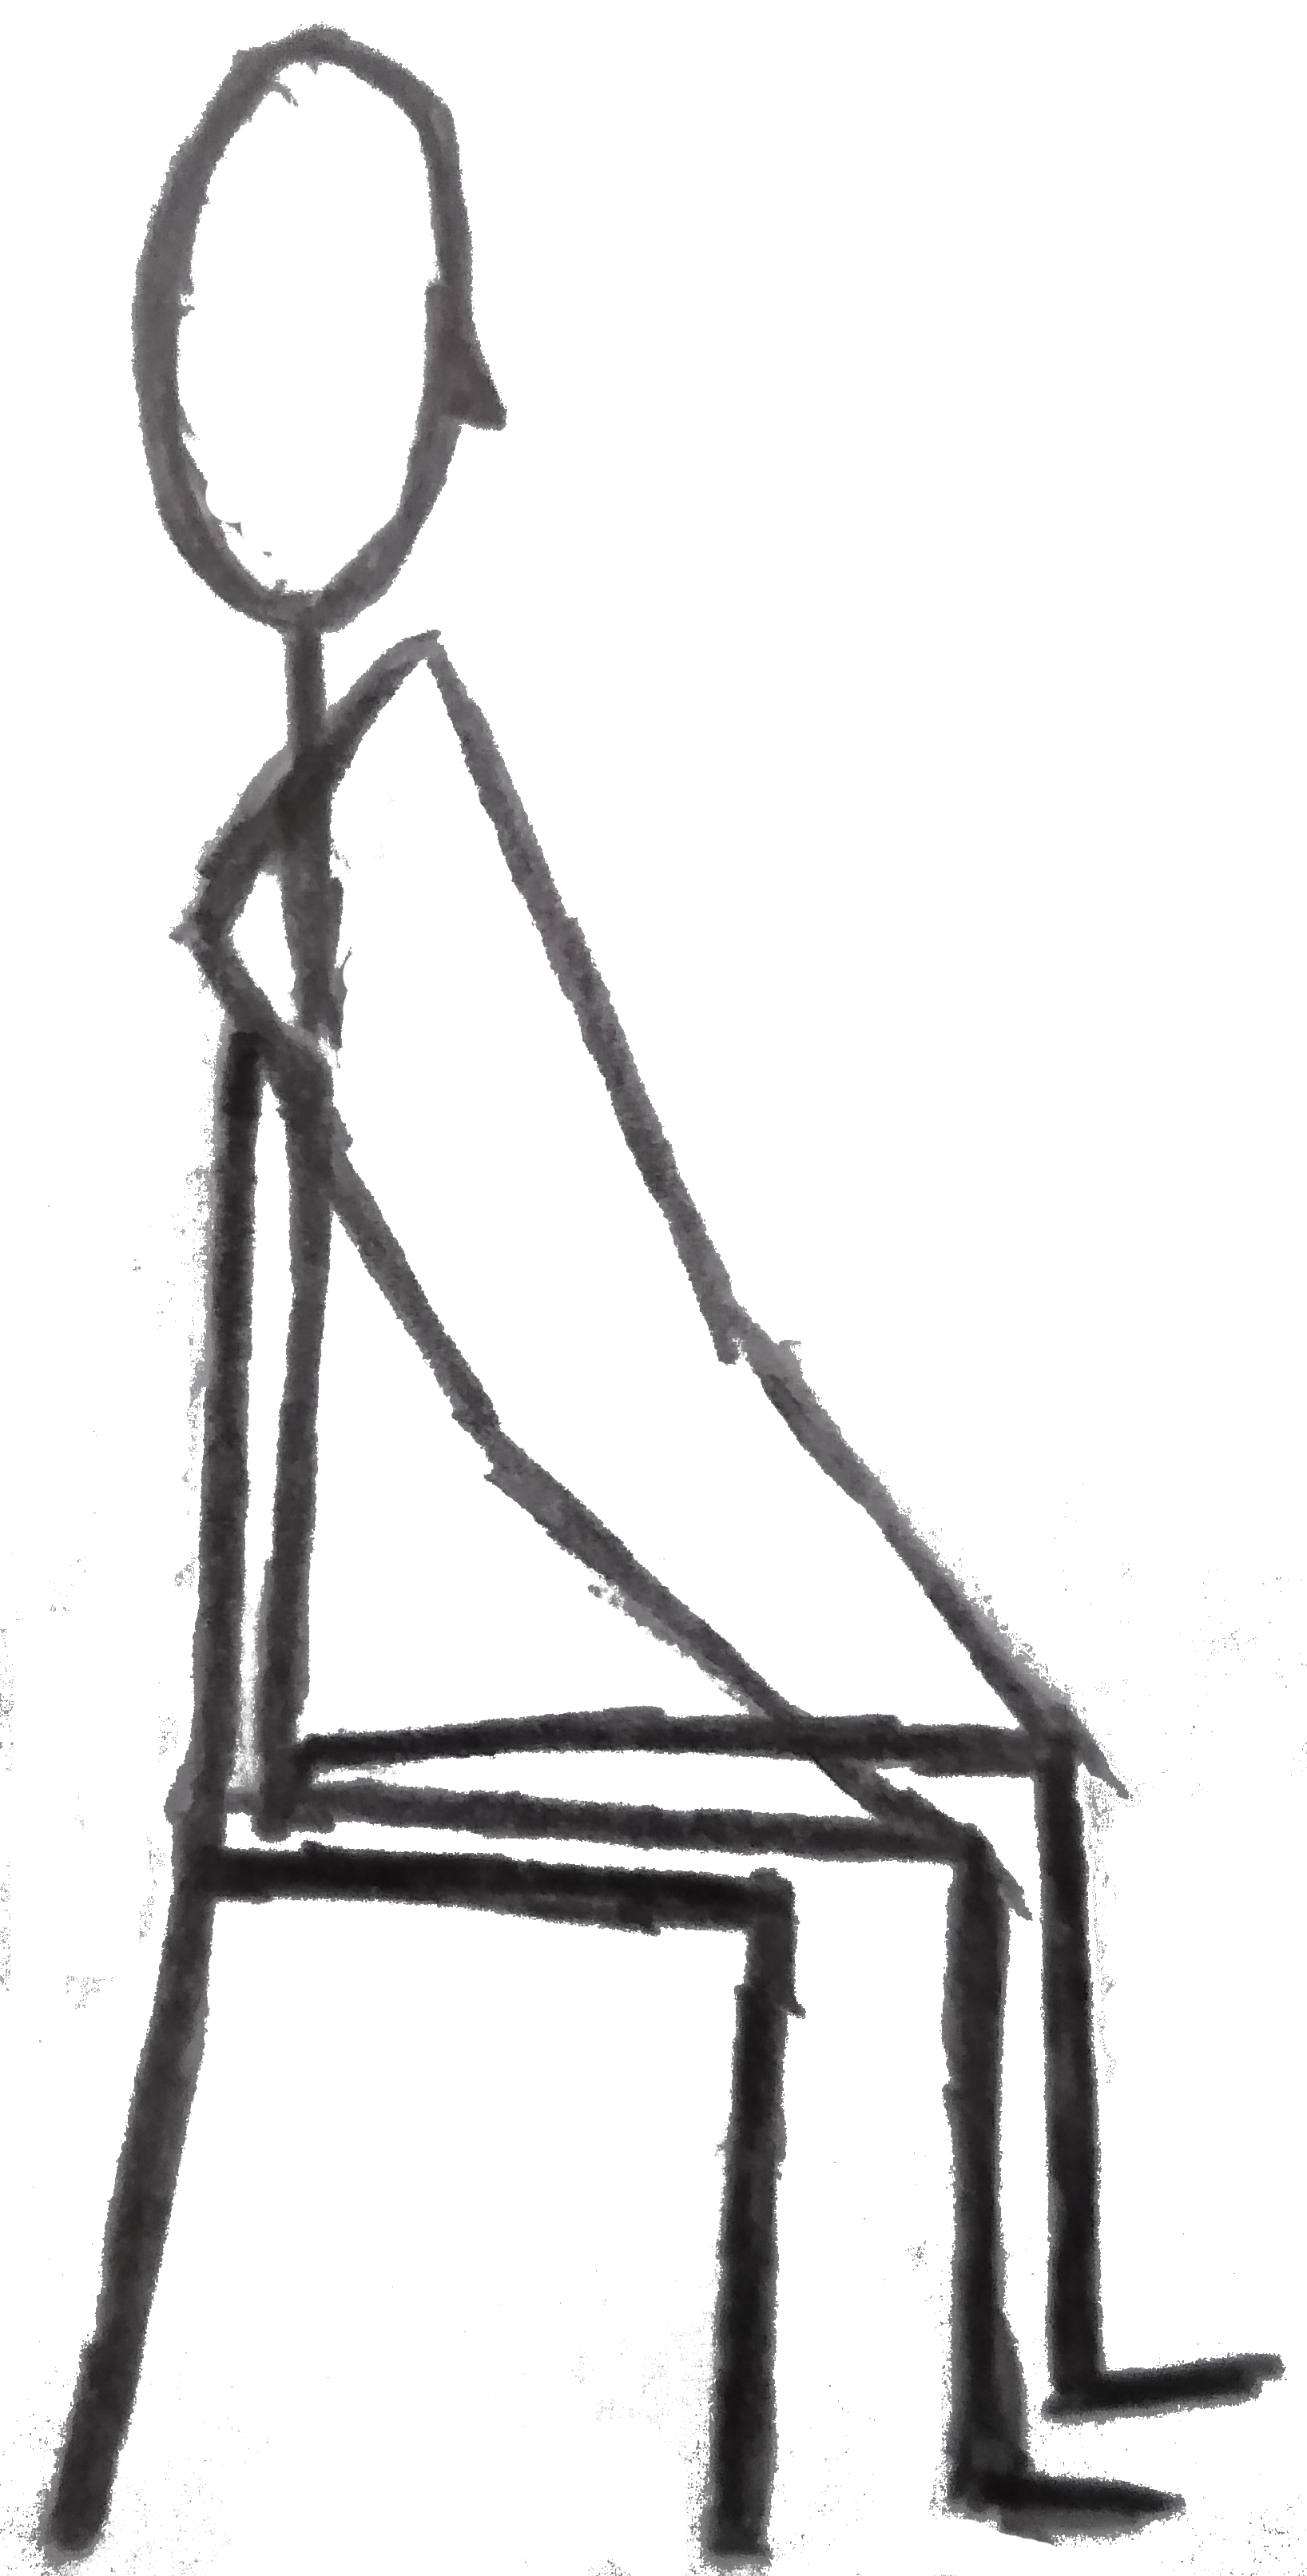
\includegraphics[width=\linewidth]{Sitting_chair_side.png}
\column{.7\textwidth} % Right column and width
\begin{itemize}
\item[-] Promotes general \structure{relaxation} (by the \structure{high performance pressure}, a lot of people have a hard time relaxing).
\item[-] Decrease of too high \structure{muscle tension}, that promotes the \structure{energy flow}.
\item[-] The \structure{brain} gets supplied with energy, which leads to an optimisation of the \structure{sleep quality}.
\item[-] \structure{Evening depressions} disappear.
\item[-] Healthy \structure{sexuality} gets promoted. % Depending on, comment out
\end{itemize}
% Write on
\end{columns}
\end{frame}
%--------------------------------------------------------------------------------------------------------------
%--------------------------------------------------------------------------------------------------------------
\begin{frame}
\frametitle{Possible morning program}
\begin{columns}[c] % The "c" option specifies centered vertical alignment while the "t" option is used for top vertical alignment

\column{.3\textwidth} % Left column and width
%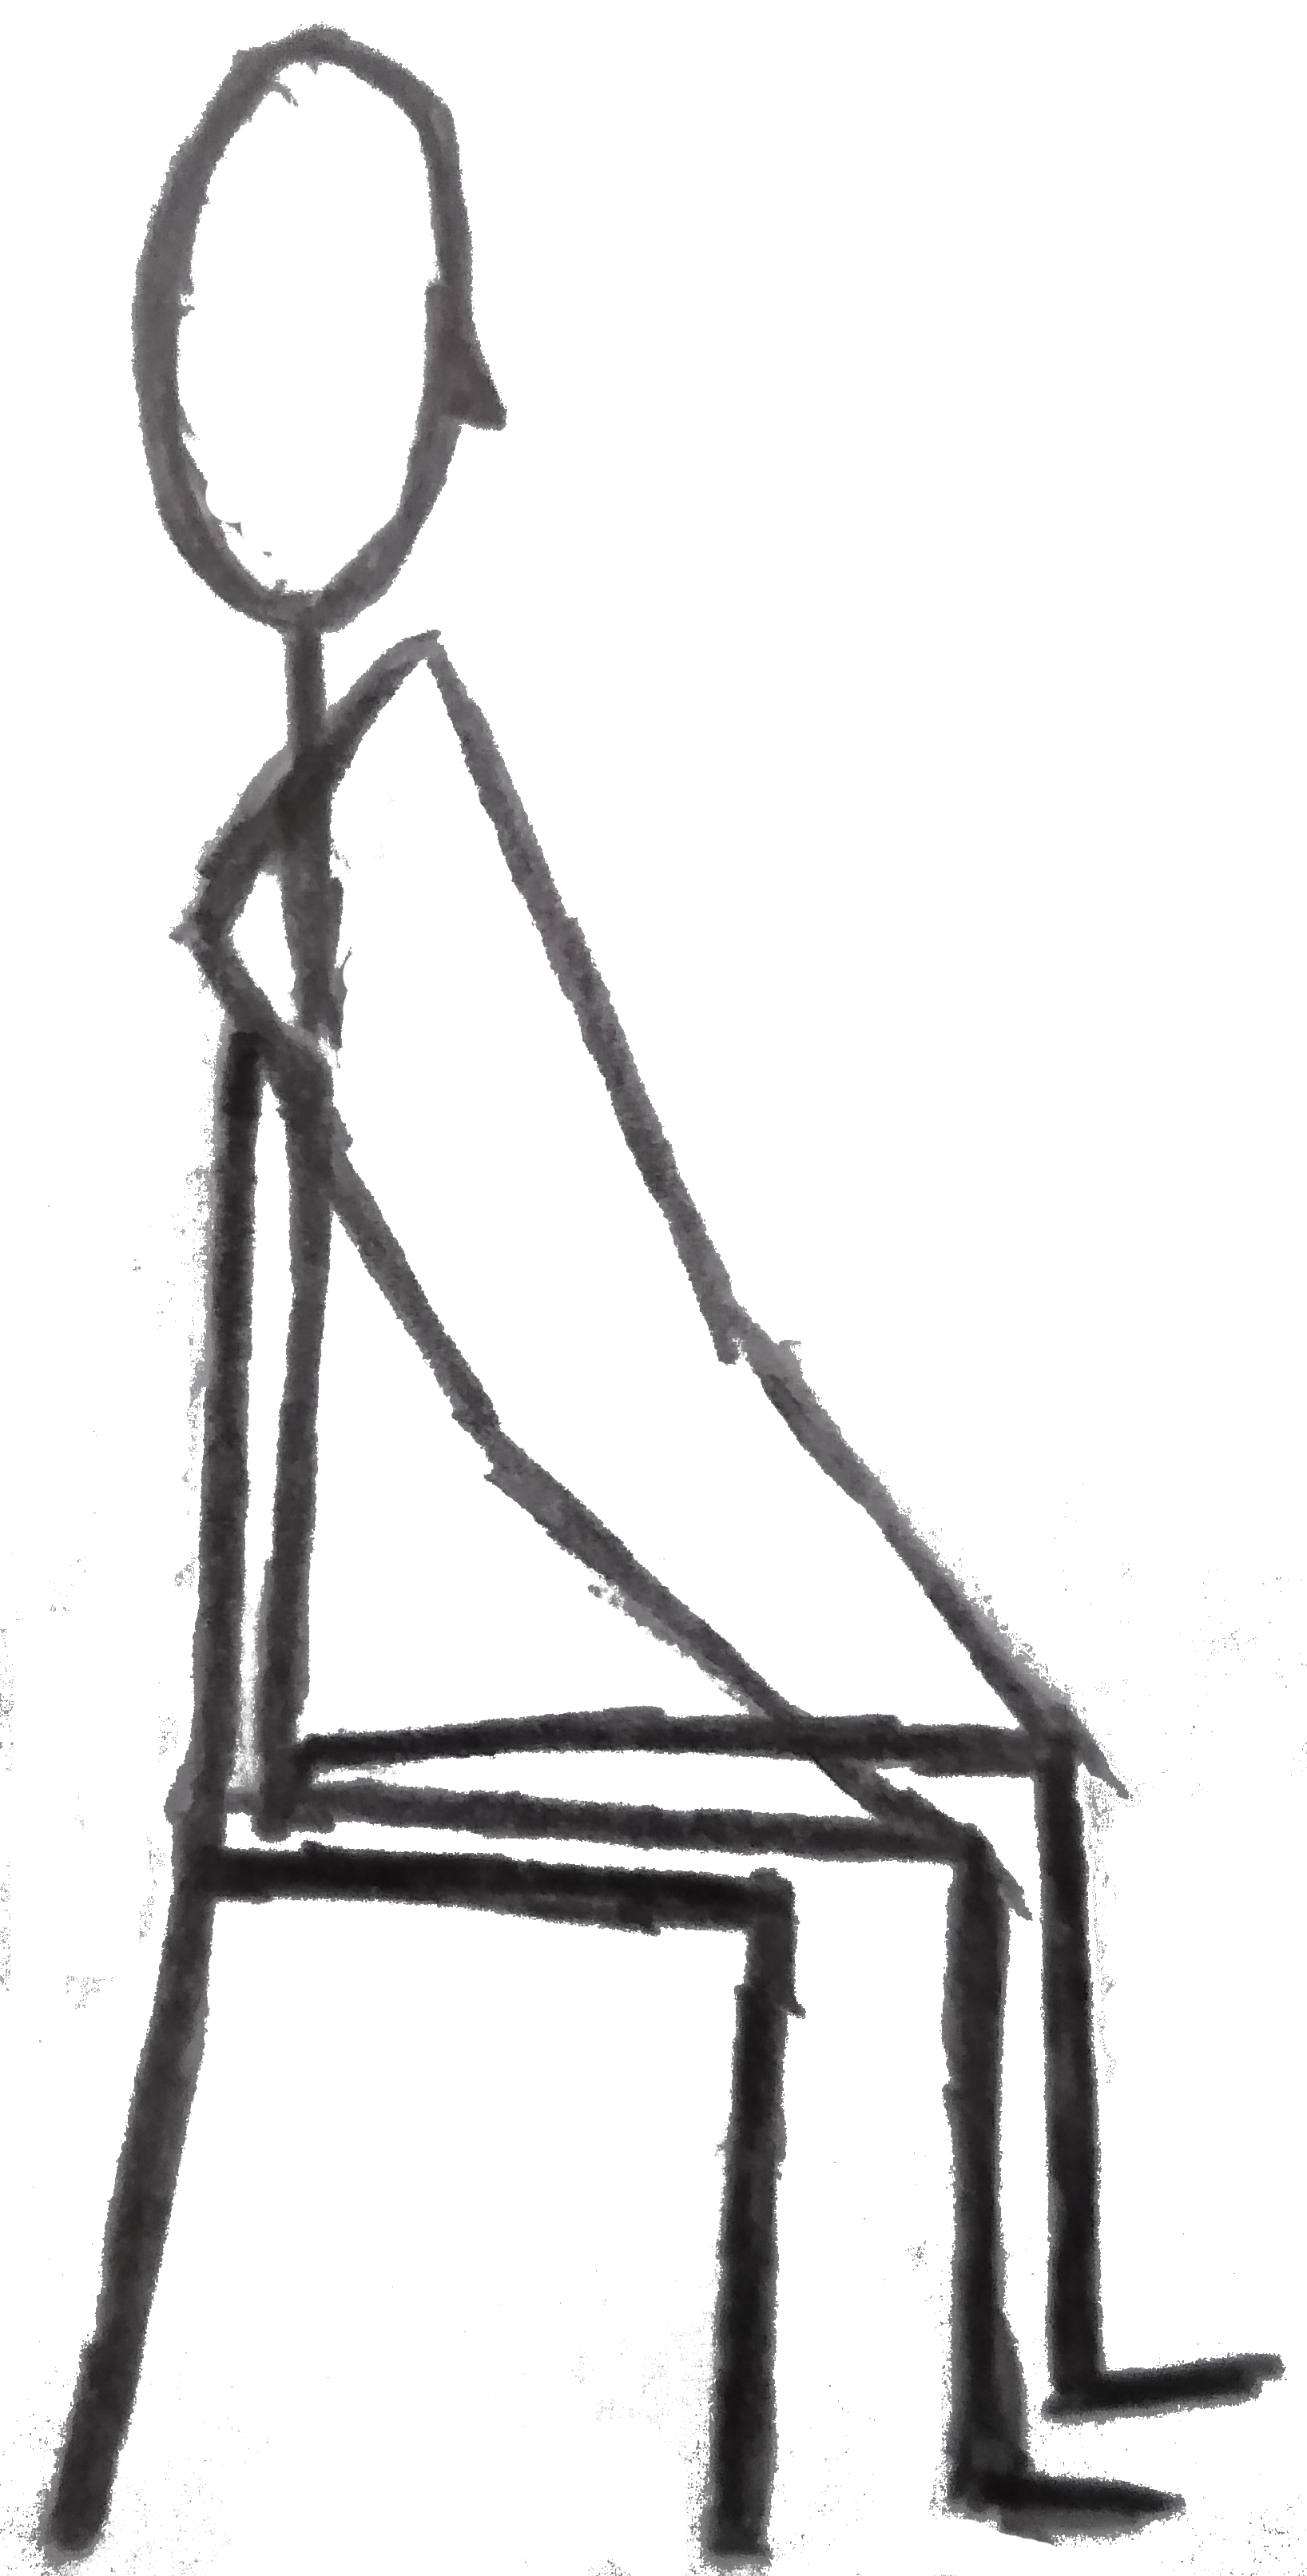
\includegraphics[width=\linewidth]{Sitting_chair_side.png}
\column{.7\textwidth} % Right column and width
\begin{itemize}
\item[-] Possibly \underline{\structure{central pillar}} %(?) %Maybe comment out if I don't write it up
before getting out of bed
\item[-] Drink \structure{water} (possibly warm/ with lemon)
\item[-] Sit down to \structure{rest the brain} (\underline{Big hug}, %Maybe comment out if I don't write it up
\underline{heart coherence exercise}, 
\underline{finger holding}, %Maybe comment out if I don't write it up
\underline{sitting meditation})
\item[-] \underline{Sun salutation}, \underline{Rune exercises}, \underline{Meridian exercises}, %Maybe comment out if I don't write it up
\underline{7 Tibetans} %Maybe comment out if I don't write it up, I have 2
\item[-] \underline{PCE training}
\end{itemize}
% Write on
\end{columns}
\end{frame}
%--------------------------------------------------------------------------------------------------------------
\begin{frame}
\frametitle{Possible evening program}
\begin{columns}[c] % The "c" option specifies centered vertical alignment while the "t" option is used for top vertical alignment

\column{.3\textwidth} % Left column and width
%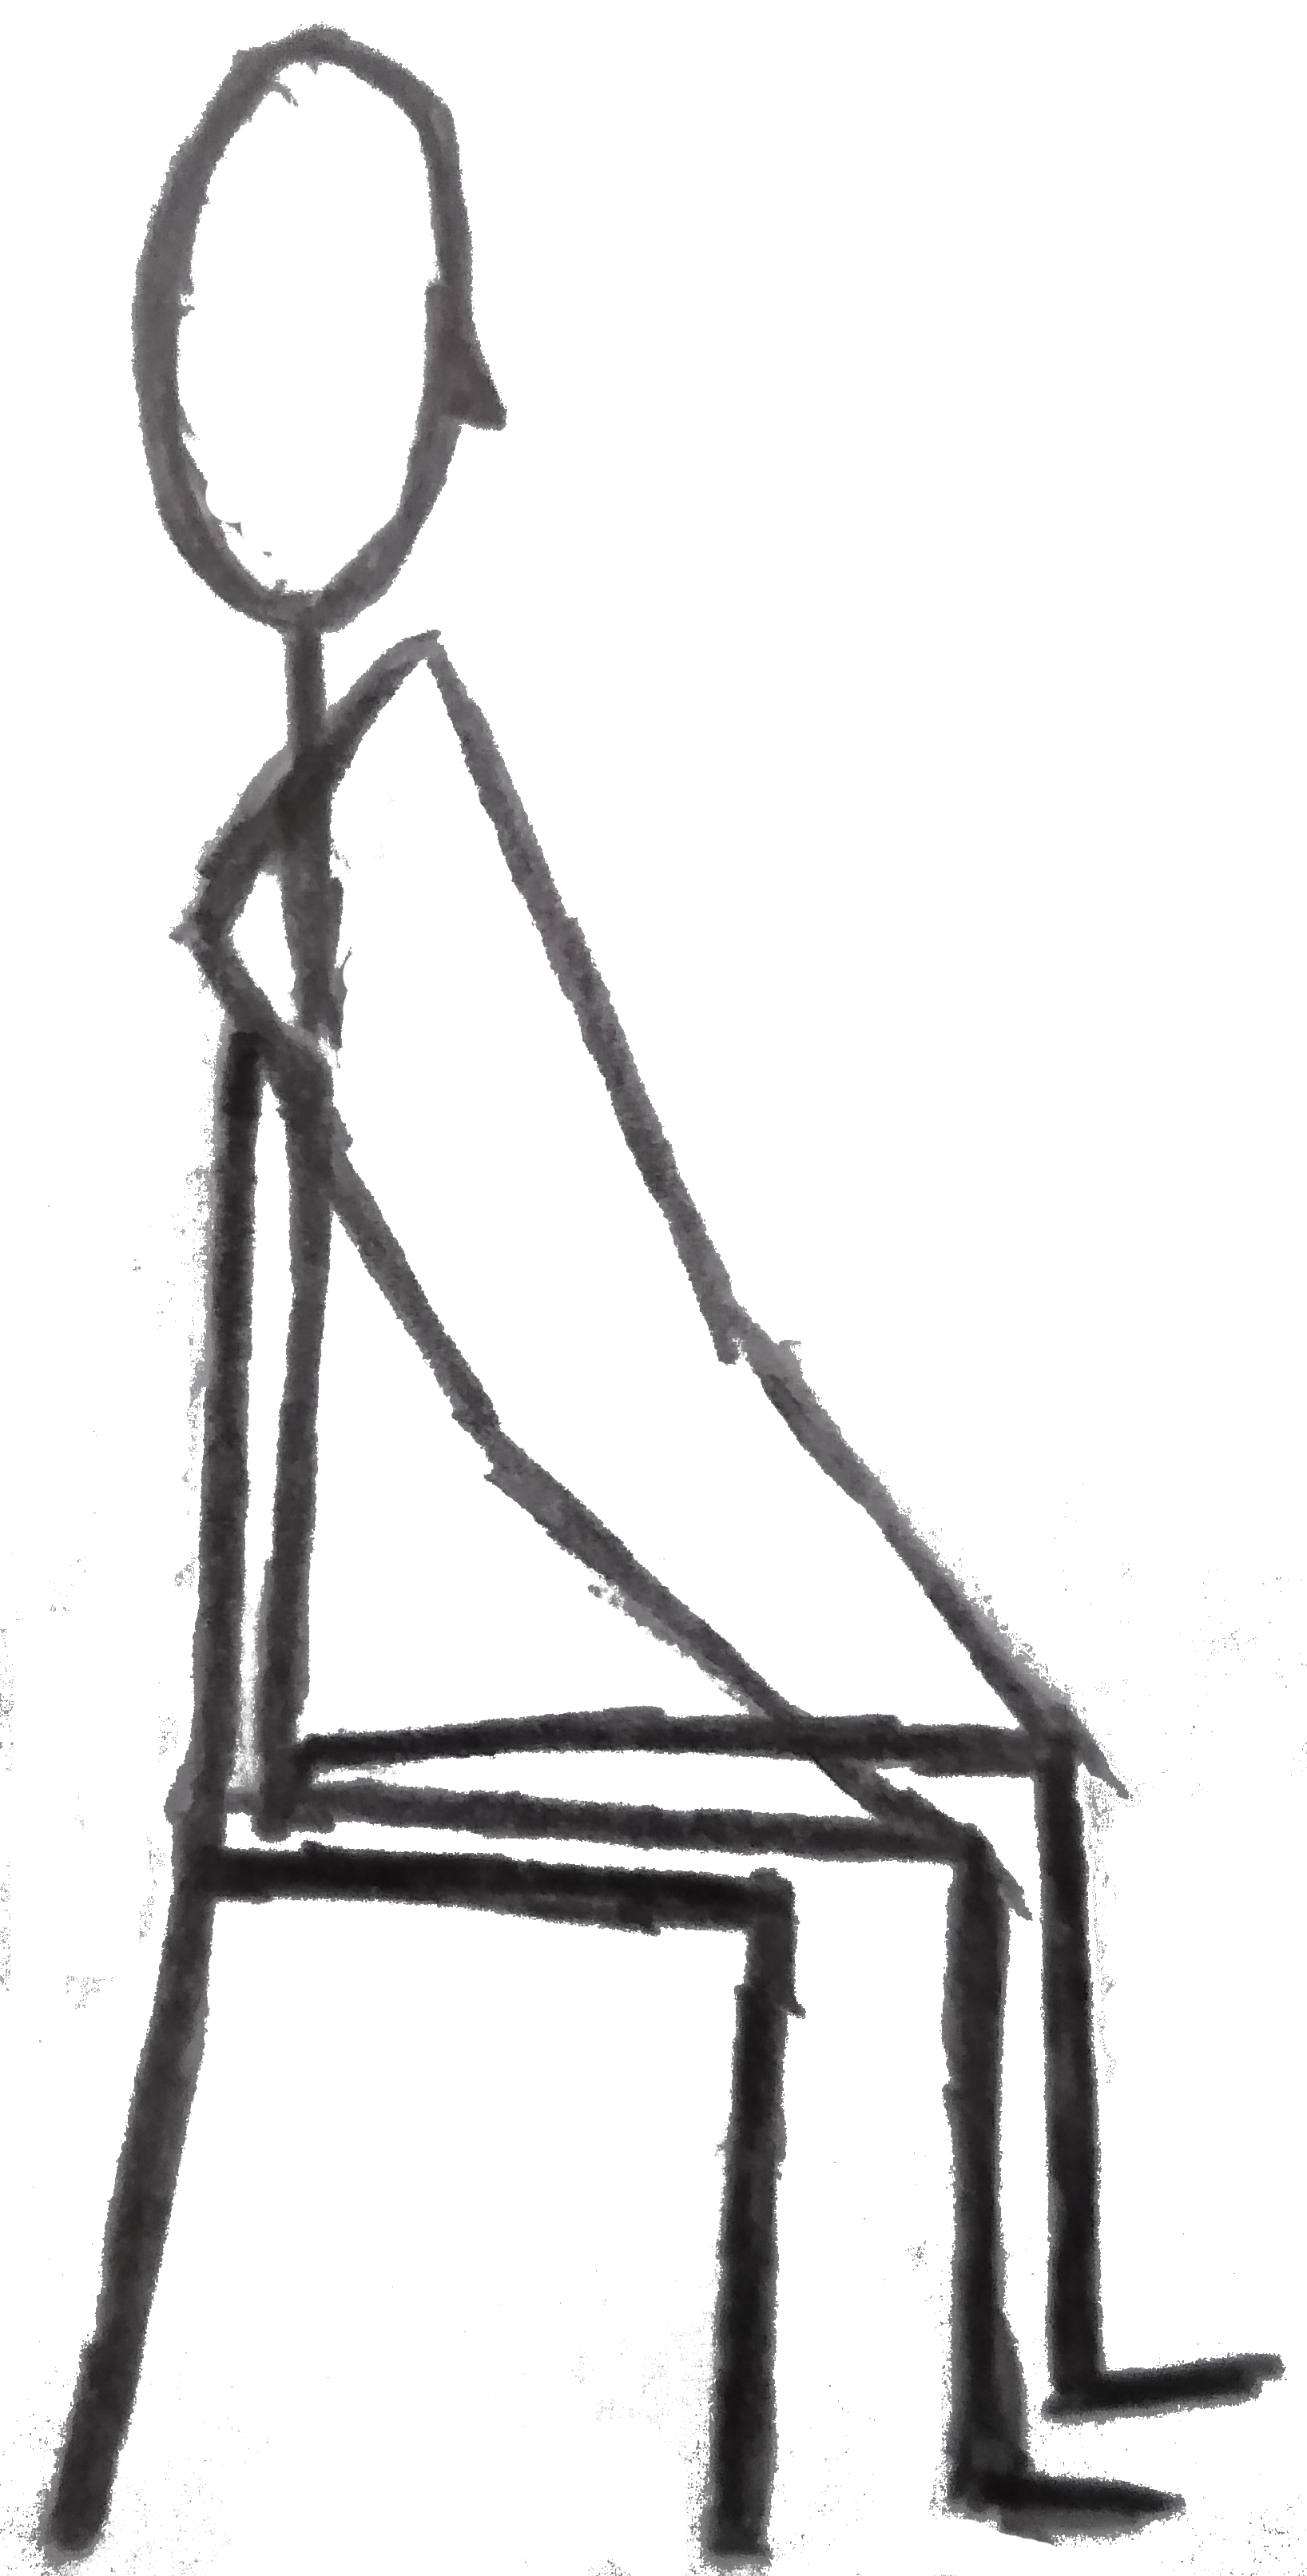
\includegraphics[width=\linewidth]{Sitting_chair_side.png}
\column{.7\textwidth} % Right column and width
\begin{itemize}
\item[-] \structure{Never go straight from performance to bed} (work, read, tv, discussion,\ldots)
\item[-] Eventually an \structure{evening walk}.
\item[-] \structure{Movement ritual}: \underline{Rune} / \underline{Meridian exercises}
\item[-] \structure{Calm exercise} (hands on lap, thumb to index -- feel the pulse and count to 50 or: \underline{heart coherence}, \underline{big hug}, 
\underline{spleen stream}, % Maybe comment out, I think Shi Shin Jitsu
\underline{sitting meditation}) 
\item[-] \underline{PCE training} 10x, tongue on roof of mouth, close your eyes, looking up to the root of the nose
\end{itemize}
% Write on
\end{columns}
\end{frame}
%--------------------------------------------------------------------------------------------------------------
